\documentclass[12pt]{article}
\usepackage{mathtext}
\usepackage{amsmath}
\usepackage[T2A]{fontenc}
\usepackage[utf8]{inputenc}
\usepackage[russian]{babel}
\usepackage[left=1.5cm, right=1.5cm, top=2cm, bottom=2cm, bindingoffset=0cm]{geometry}
\usepackage{listings}
\usepackage{fancyhdr}
\usepackage{pgfplots}
\pgfplotsset{compat=1.9}



\begin{document}
    \begin{center}
        \textbf{Московский авиационный институт} \\
        \textbf{(Национальный исследовательский университет)}
    \end{center} 
    ~\\
    ~\\
    Институт: «Информационные технологии и прикладная математика» \\
    Кафедра: 805 «Математическая кибернетика»  \\
    Дисциплина: «Численные методы»  
    ~\\
    ~\\
    ~\\
    \begin{center}
        Лабораторная работа №4 \\
        Тема: Решение двумерной начально-краевой задачи для дифференциального\\ уравнения 
        параболического типа
    \end{center}
    ~\\
    ~\\
    ~\\
    ~\\
    ~\\
    ~\\
    ~\\
    ~\\
    ~\\
    \begin{flushright}
        Студент: ~~~~~~~~~~~~Хахин Максим~~~~~~\\
        Группа: ~~~~~~~~~~~~~~80-403~~~~~~~~~~~~~~~~~\\
        Преподаватель: ~~~~Иванов И. Э.~~~~~~~\\
        Дата: ~~~~~~~~~~~~~~~~~~~~~~~~~~~~~~~~~~~~~~~~~~~\\
        Оценка: ~~~~~~~~~~~~~~~~~~~~~~~~~~~~~~~~~~~~~~~~\\
    \end{flushright}
    ~\\
    ~\\
    ~\\
    ~\\
    ~\\
    ~\\
    ~\\
    ~\\
    ~\\
    ~\\
    ~\\
    ~\\
    ~\\
    ~\\
    ~\\
    \begin{center}
        Москва, 2021
    \end{center}
    \pagestyle{empty}
    \newpage

    \pagestyle{fancy} 
        \fancyhead{}
        \fancyhead[L]{Хахин Максим}
        \fancyhead[R]{М8О-403Б-18} 
    \fancyfoot{} 
    \begin{enumerate}
        \item \textbf{Задание:}\\
        Используя явную и неявную конечно-разностные схемы, а также схему Кранка - Николсона, решить начально-краевую задачу для дифференциального уравнения параболического типа. Осуществить реализацию трех вариантов аппроксимации граничных условий, содержащих производные: двухточечная аппроксимация с первым порядком, трехточечная аппроксимация со вторым порядком, двухточечная аппроксимация со вторым порядком. В различные моменты времени вычислить погрешность численного решения путем сравнения результатов с приведенным в задании аналитическим решением. Исследовать зависимость погрешности от сеточных параметров.

        \item \textbf{Вариант 8:}\\
        \begin{figure}[h]
            \center{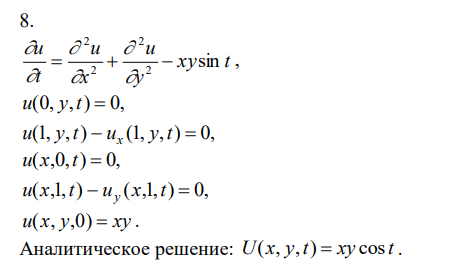
\includegraphics[width=0.5\linewidth]{ 1.png}}
            \label{ris:image}
        \end{figure}\\
        \item \textbf{Теория:}\\
         При численном решении многомерных задач математической физики
        исключительно важным является вопрос об экономичности используемых
        методов. Конечно - разностную схему будем называть экономичной, если
        число выполняемых операций (операций типа умножения) пропорционально
        числу узлов сетки. 
        \\За последние 50 лет разработано значительное количество
        экономичных разностных схем численного решения многомерных задач
        математической физики, основанных на расщеплении пространственных
        дифференциальных операторов по координатным направлениям и
        использовании метода скалярной прогонки вдоль этих направлений. 
        \\Из экономичных конечно-разностных схем, получивших наибольшее
        распространение, в данном разделе рассматриваются схема метода
        переменных направлений и схема метода дробных шагов. Все эти методы
        будем называть общим термином - методы расщепления.
        \\Для начала необходимо ввести пространственно-временную сетку:
        $$\omega^{\tau}_{h_1h_2} = \{ x_i = ih_1, i=\overline{0,I}, j=\overline{0,J} : 
        t^k = k\tau, k = 0,1,2...\} $$
        Рассмотрим методы решения
        \\Метод переменных направлений
        \\Шаг по времени разбивается на число независимых переменных. На каждом 
        дробном слое один из операторов аппроксимируется неявно, а другой 
        явно. Вид для двумерного случая:
        $$u^{k+1/2}_{ij} - u^k_{ij}= \sigma_x(u^{k+1/2}_{i+1 j}-2u^{k+1/2}_{i j} +u^{k+1/2}_{i-1 j})+
        \sigma_y(u^{k}_{i j+1} - 2u^{k}_{i j} + u^{k}_{i j-1}) + f^{k+1/2}_{ij}(\tau/2)$$
        $$u^{k+1}_{ij} - u^{k+1/2}_{ij}= \sigma_x(u^{k+1/2}_{i+1 j}-2u^{k+1/2}_{i j} +u^{k+1/2}_{i-1 j})+
        \sigma_y(u^{k+1}_{i j+1} - 2u^{k+1}_{i j} + u^{k+1}_{i j-1}) + f^{k+1/2}_{ij}(\tau/2)$$
        $$\sigma_x = \frac{a\tau}{2h^2_x},~\sigma_y = \frac{a\tau}{2h^2_y}$$
        $$\frac{u^{k+1/2}_{ij} - u^k_{ij}}{\tau/2}= \frac{a}{h_x^2}(u^{k+1/2}_{i+1 j}-2u^{k+1/2}_{i j} +u^{k+1/2}_{i-1 j})+
        \frac{a}{h_y^2}(u^{k}_{i j+1} - 2u^{k}_{i j} + u^{k}_{i j-1}) + h_{xi}h_{yj} cos(\tau(k+1/2))$$
        $$u_{ij}^{k+1/2} = \frac{\frac{2}{\tau} u_{ij}^{k} + \frac{a}{h_x^2} (u_{i+1 j}^{k+1/2}+u_{i-1 j}^{k+1/2})
        + \frac{a}{h_y^2} (u_{ij+1}^k -2u_{ij}^k+u_{ij-1}^k )+h_{xi}h_{yj}cos(\tau(k+1/2)) 
        }{2\left(\frac{1}{\tau} + \frac{a}{h_x^2}\right)}$$
        $$u_{ij}^{k+1} = \frac{\frac{2}{\tau} u_{ij}^{k +1/2} + \frac{a}{h_x^2} (u_{i+1j}^{k+1/2} -2u_{ij}^{k+1/2}+u_{i-1j}^{k+1/2})
        + \frac{a}{h_y^2} (u_{i j+1}^{k+1}+u_{i j+1}^{k+1} )+h_{xi}h_{yj}cos(\tau(k+1/2)) 
        }{2\left(\frac{1}{\tau} + \frac{a}{h_x^2}\right)}$$

        
        \item \textbf{Код:}\\
        \begin{lstlisting}[language=python]
            \\Define the initial boundary conditions
a = 1
b = 1

lx = 1
ly = 1
lt = 5
omega = 1.5
nx = 100
ny = 100
nt = 100
eps = 0.001

u0yt = lambda y, t: 0
ulyt = lambda y, t: 0
ux0t = lambda x, t: 0
uxlt = lambda x, t: 0
uxy0 = lambda x, y: x*y
f = lambda x, y, t: -x*y*np.sin(t)

fResult = lambda x, y, t: x*y*np.cos(t)

alpha1 = 1
betta1 = -1
alpha2 = 1
betta2 = -1


            \\FractionSteps and AlternatingDirection


def parabolicEquation2D(iCond, bCond, method):

def init():
    for m in range(nx):
        for n in range(ny):
            U[0][m][n] = uxy0(m * hx, n * hy)

def solve():
    for k in range(0, nt - i, i):
        for n in range(1, ny - 1):
            A1 = getA1(k, n)
            B1 = getB1(k, n)
            U[int(k + i / 2), :, n] = np.linalg.solve(A1, B1)[:, 0]
        for m in range(1, nx - 1):
            A2 = getA2(k, m)
            B2 = getB2(k, m)
            U[k + i, m, :] = np.linalg.solve(A2, B2)[:, 0]
        for n in range(0, ny):
            U[k + i][0][n] = (u0yt(n * hy, (k + i) * ht) - c1 * 
             U[k + i][1][n]) / b1
            U[k + i][nx - 1][n] = (ulyt(n * hy, (k + i) * ht) - aN1 *
             U[k + i][nx - 2][n]) / bN1

def FractionSteps():

    aj1 = -a/hx**2
    bj1 = 1/ht/2 + 2*a/hx**2
    cj1 = -a/hx**2

    aj2 = -b/hy**2
    bj2 = 1/ht/2 + 2*b/hy**2
    cj2 = -b/hy**2

    def gA1(k, n):
        aa = np.zeros((nx, nx))
        aa[0][0] = b1
        aa[0][1] = c1
        for j in range(1, nx - 1):
            aa[j][j - 1] = aj1
            aa[j][j] = bj1
            aa[j][j + 1] = cj1
        aa[nx - 1][nx - 2] = aN1
        aa[nx - 1][nx - 1] = bN1
        return aa

    def gB1(k, n):
        bb = np.zeros((nx, 1))
        bb[0][0] = u0yt(n * hy, ht * (k + i))
        bb[nx - 1][0] = ulyt(n * hy, ht * (k + i))
        for m in range(1, nx - 1):
            bb[m][0] = f(m * hx, n * hy, k * ht)/2 + 
             U[k][m][n] / ht / 2
        return bb

    def gA2(k, m):
        aa = np.zeros((ny, ny))
        aa[0][0] = b2
        aa[0][1] = c2
        for j in range(1, ny - 1):
            aa[j][j - 1] = aj2
            aa[j][j] = bj2
            aa[j][j + 1] = cj2
        aa[ny - 1][ny - 2] = aN2
        aa[ny - 1][ny - 1] = bN2
        return aa

    def gB2(k, m):
        bb = np.zeros((ny, 1))
        bb[0][0] = ux0t(m * hx, ht * (k + i))
        bb[ny - 1][0] = uxlt(m * hx, ht * (k + i))
        for n in range(1, ny - 1):
            bb[n][0] = f(m * hx, n * hy, (k + i) * ht)/2 +
             U[int(k + i/2)][m][n] / ht / 2
        return bb
    return (gA1, gB1), (gA2, gB2)

def AlternatingDirection():

    aj1 = -a / hx ** 2
    bj1 = 1 / ht + 2 * a / hx ** 2
    cj1 = -a / hx ** 2

    aj2 = -b / hy ** 2
    bj2 = 1 / ht + 2 * b / hy ** 2
    cj2 = -b / hy ** 2

    def gA1(k, n):
        aa = np.zeros((nx, nx))
        aa[0][0] = b1
        aa[0][1] = c1
        for j in range(1, nx - 1):
            aa[j][j - 1] = aj1
            aa[j][j] = bj1
            aa[j][j + 1] = cj1
        aa[nx - 1][nx - 2] = aN1
        aa[nx - 1][nx - 1] = bN1
        return aa

    def gB1(k, n):
        bb = np.zeros((nx, 1))
        bb[0][0] = u0yt(n * hy, ht * (k + i))
        bb[nx - 1][0] = ulyt(n * hy, ht * (k + i))
        for m in range(1, nx - 1):
            bb[m][0] = f(m * hx, n * hy, int(k + i/2) * ht) + 
             (1 / ht - 2*b/ hy**2) * U[k][m][n] + (b/hy**2) *
              (U[k][m][n + 1] + U[k][m][n - 1])
        return bb

    def gA2(k, m):
        aa = np.zeros((ny, ny))
        aa[0][0] = b2
        aa[0][1] = c2
        for j in range(1, ny - 1):
            aa[j][j - 1] = aj2
            aa[j][j] = bj2
            aa[j][j + 1] = cj2
        aa[ny - 1][ny - 2] = aN2
        aa[ny - 1][ny - 1] = bN2
        return aa

    def gB2(k, m):
        bb = np.zeros((ny, 1))
        bb[0][0] = ux0t(m * hx, ht * (k + i))
        bb[ny - 1][0] = uxlt(m * hx, ht * (k + i))
        for n in range(1, ny - 1):
            bb[n][0] = f(m * hx, n * hy, int(k + i/2) * ht) +
             (1 / ht - 2*a/ hx**2) * U[int(k + i/2)][m][n] +
              (a/hx**2) * (U[int(k + i/2)][m + 1][n] + 
              U[int(k + i/2)][m - 1][n])
        return bb

    return (gA1, gB1), (gA2, gB2)
if method == 1:
    (getA1, getB1), (getA2, getB2) = AlternatingDirection()
elif method == 2:
    (getA1, getB1), (getA2, getB2) = FractionSteps()
else:
    pass
b1 = 1
c1 = 0
b2 = 1
c2 = 0

aN1 = -betta1 / hx
bN1 = alpha1 + betta1 / hx
aN2 = -betta2 / hy
bN2 = alpha2 + betta2 / hy

uxy0 = iCond
xCond, yCond = bCond
u0yt, ulyt = xCond
ux0t, uxlt = yCond
U = gridFun((0, nt), ((0, nx), (0, ny)))
i = 2
init()
solve()
return U



            \end{lstlisting}
        
        \item \textbf{Результат:}\\
        Метод дробных шагов:

        \begin{figure}[h]
            \center{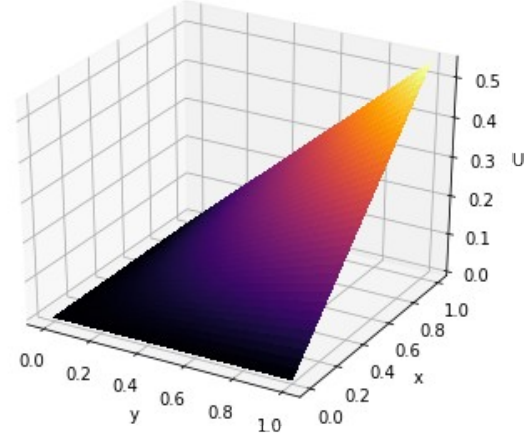
\includegraphics[width=0.5\linewidth]{ 2.png}}
            \label{ris:image}
        \end{figure}\\
        \newpage
        График зависимости ошибки от размера шага по пространству:
        \begin{figure}[h]
            \center{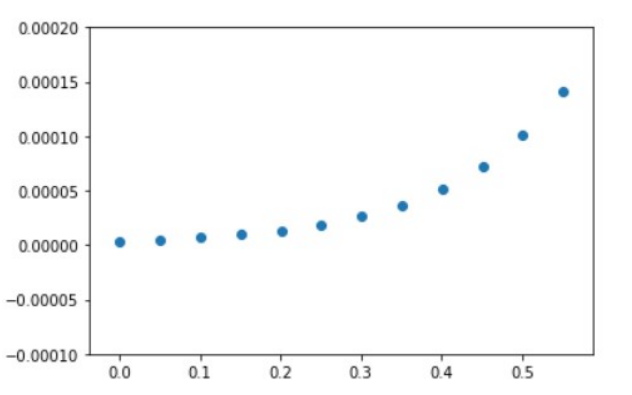
\includegraphics[width=0.5\linewidth]{ 3.png}}
            \label{ris:image}
        \end{figure}\\
        Метод переменных направлений:
        \begin{figure}[h]
            \center{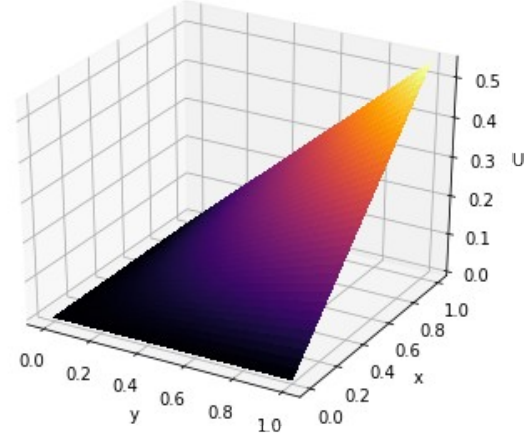
\includegraphics[width=0.4\linewidth]{ 2.png}}
            \label{ris:image}
        \end{figure}\\
        \newpage
        График зависимости ошибки от размера шага по пространству:
        \begin{figure}[h]
            \center{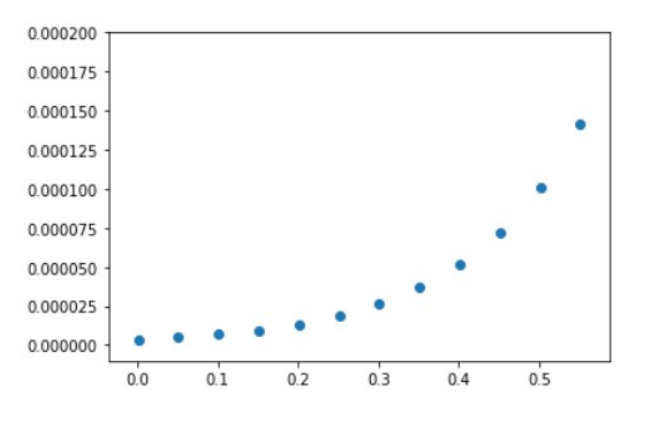
\includegraphics[width=0.5\linewidth]{ 4.png}}
            \label{ris:image}
        \end{figure}\\



        
        \item \textbf{Вывод:}\\
        Используя схемы переменных направлений и дробных шагов, научился
        решать двумерную начально-краевую задачу для дифференциального 
        уравнения параболического типа
    \end{enumerate}
\end{document}